% this file is called up by thesis.tex
% content in this file will be fed into the main document

%: ----------------------- name of chapter  -------------------------
\chapter{Projekt i implementacja systemu SpeechProcessingPlatform} % top level followed by section, subsection


%: ----------------------- paths to graphics ------------------------

% change according to folder and file names
\ifpdf
    \graphicspath{{6/figures/PNG/}{6/figures/PDF/}{6/figures/}}
\else
    \graphicspath{{6/figures/EPS/}{6/figures/}}
\fi

%: ----------------------- contents from here ------------------------

Rozdział ten opisuje architekturę, projekt i implementację przykładowej platformy integracyjnej SpeechProcessingPlatform, która umożliwi weryfikację proponowanego podejścia. Platforma ta jest projektowana z myślą o architekturze opartej na technologii ESB, którą autorzy uznali za najlepiej nadającą się do realizacji systemów integracyjnych. Rozdział ten zawiera opis najważniejszych części systemu, zależności między nimi oraz formatu danych wykorzystywanego w komunikacji.

\section{Architektura}

Rysunek \ref{fig:layered_architecture} przedstawia architekturę systemu SpeechProcessingPlatform. Jest ona podzielona na 3 warstwy:

\begin{itemize}
	\item Data Endpoints Layer
	\item Routing Layer
	\item Services Layer
\end{itemize}

\begin{figure}[!h]
	\centering
	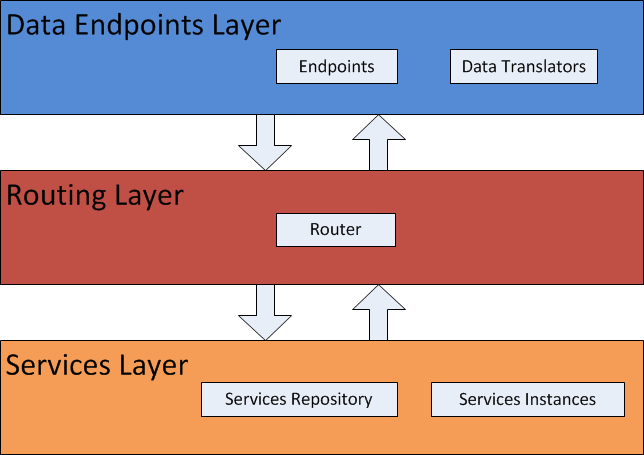
\includegraphics[scale=0.7]{layered_architecture.png}
	\caption{Architektura systemu SpeechProcessingPlatform}\label{fig:layered_architecture}
\end{figure}

Podejście warstwowe ułatwia dekompozycję systemu na niezależne komponenty, które odpowiadają za dobrze zdefiniowany fragment wymaganej funkcjonalności. 
% tu mozna cos dodac jak cos

Warstwa \textit{Data Endpoints Layer} odpowiada za udostępnianie interfejsów dla aplikacji klienckich oraz za transformacje danych do wspólnego formatu. Głównymi elementami tej warstwy są punkty końcowe i translatory danych. Punkty końcowe wystawiają interfejsy umożliwiające dostęp do platformy przy użyciu różnych technologii takich jak REST, FTP, SOAP czy RSS. Zadaniem translatorów jest ujednolicenie danych do postaci używanej w kolejnych warstwach. Dzięki temu komponenty z warstw niższych mają uproszczoną implementację ponieważ skupiają się na obsłudze tylko jednego, dobrze zdefiniowanego formatu. 

Warstwa \textit{Routing Layer} odpowiada za routowanie zadań przetwarzania od punktów końcowych do odpowiednich komponentów udostępniających usługi przetwarzania mowy, a także za przesyłanie wyników z powrotem do punktów końcowych. Zadania mogą być jedno etapowe jak np. \textit{przetłumacz ten tekst z języka polskiego na język angielski} albo dwu lub więcej etapowe jak np. \textit{rozpoznaj tekst na tym zdjęciu, jeżeli trzeba przetłumacz na język angielski i na jego podstawie wygeneruj dźwięk}.

Głównym elementami ostatniej warstwy, \textit{Services Layer}, jest repozytorium komponentów odpowiadających za przetwarzanie mowy oraz konkretne ich instancje. Główne zadanie repozytorium to wyszukiwanie i zwracanie odpowiednich instancji w odpowiedzi na żądania warstwy routującej. Najważniejszą cechą wyróżniającą poszczególne komponenty jest typ przetwarzania mowy jaki dostarczają. Ze względu na to kryterium zostały one podzielone na 5 grup, a każda z nich posiada dodatkowe cechy, które także mają wpływ na wynik wyszukiwania:

\begin{itemize}
	\item OCR
	\begin{itemize}
		\item wejście - plik graficzny, parametry:
		\begin{itemize}
			\item obsługiwane języki 
			\item obsługiwane formaty plików
		\end{itemize}
		\item wyjście - plik tekstowy
	\end{itemize}
	\item ASR
	\begin{itemize}
		\item wejście - plik dźwiękowy, parametry:
		\begin{itemize}
			\item obsługiwane języki 
			\item obsługiwane formaty plików
		\end{itemize}
		\item wyjście - plik tekstowy
	\end{itemize}
	\item TTS
	\begin{itemize}
		\item wejście - plik tekstowy, parametry:
		\begin{itemize}
			\item obsługiwane języki 
			\item obsługiwane formaty wyjściowe
			\item obsługiwane formaty znaczników
		\end{itemize}
		\item wyjście - plik dźwiękowy, parametry:
		\begin{itemize}
			\item obsługiwane formaty plików
		\end{itemize}
	\end{itemize}
	\item translacja
	\begin{itemize}
		\item wejście - plik tekstowy, parametry:
		\begin{itemize}
			\item obsługiwane języki 
		\end{itemize}
		\item wyjście - plik tekstowy
	\end{itemize}
	\item rozpoznawanie języka
	\begin{itemize}
		\item wejście - plik tekstowy
		\item wyjście - informacja o języku
	\end{itemize}
\end{itemize}

Oczywiście konkretny komponent może udostępniać więcej niż jeden typ przetwarzania np. komponent translacji może od razu być w stanie rozpoznać język źródłowy, dzięki czemu nie musi mieć tej informacji dostarczonej razem z tekstem.

\begin{figure}[!h]
	\centering
	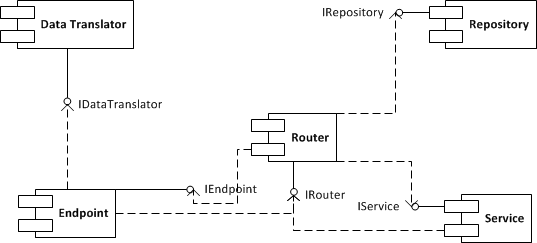
\includegraphics[scale=1.0]{component_uml.png}
	\caption{Diagram komponentów systemu SpeechProcessingPlatform w notacji UML 1.0}\label{fig:component_diagram}
\end{figure}

\section{Projekt}

Jak było wspomniane, do realizacji systemu SpeechProcessingPlatform została wybrana technologia ESB. Głównymi zaletami tej technologii są skalowalność i wysoki poziom abstrakcji, dzięki któremu budowa systemu jest ułatwiona - pozwala skupić się na problemie a nie na szczegółach implementacji. Dodatkowo, kontenery ESB dostarczają dużo użytecznych funkcjonalności takich jak: routing, transformacja danych, komunikacja oparta na wiadomościach, zestaw gotowych punktów końcowych. Wszystko to sprawia, że proces integracji jest znacznie ułatwiony. Projektowanie systemu z użyciem wiadomości jako modelu komunikacji, różni się od tradycyjnego podejścia z blokującymi wywołaniami metod. Interfejsy w postaci listy pól i metod, które dany komponent implementuje zostają zastąpione przez odpowiednie kanały wiadomości oraz format danych, które będą nimi przesyłane. Każdy komponent, który chce otrzymywać wiadomości udostępnia odpowiedni kanał pod dobrze znanym adresem, dzięki czemu inne komponenty są wstanie wysłać odpowiednie dla niego wiadomości. Dzięki użyciu tego modelu, zastosowanie dobrze sprawdzonych wzorców EIP staję się bardzo naturalne. 

\subsection{Warstwa \textit{Data Endpoints Layer}}

Ilustracja \ref{fig:endpoins_layer_project} przedstawia przepływ wiadomości w warstwie \textit{Data Endpoints Layer}. Aplikacje klienckie wysyłają żądanie przetwarzania na określony punkt końcowy, używając wybranego i obsługiwanego przez platformę protokołu. Żądania te zostają przetłumaczone na wspólny format wiadomości używany w dalszych częściach systemu, a następnie przesłane do routera. Dodatkowo, każdy punkt końcowy posiada swój indywidualny kanał odpowiedzi, którego adres jest dodawany do wiadomości jako adres zwrotny. Dzięki temu, router będzie wstanie odesłać wynik przetwarzania do odpowiedniego punktu końcowego.

\begin{figure}[!h]
	\centering
	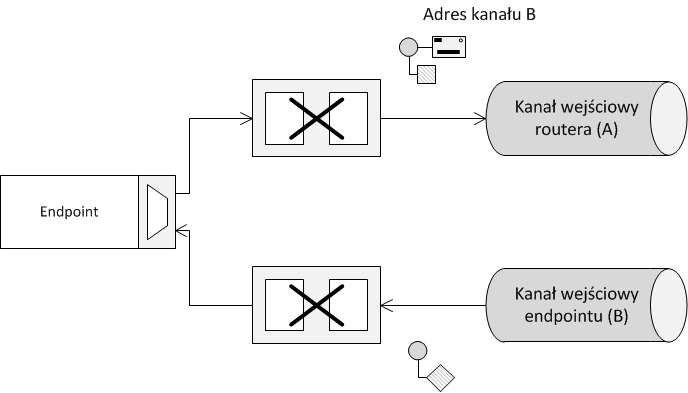
\includegraphics[scale=0.8]{endpoints_layer_flow.png}
	\caption{Diagram przepływu wiadomości w warstwie \textit{Data Endpoints Layer}}\label{fig:endpoins_layer_project}
\end{figure}

Ponieważ przetwarzanie mowy może być procesem czasochłonnym, budowana platforma powinna wspierać komunikację asynchroniczną. Niektóre punkty końcowe, takie jak FTP czy SMTP są z natury asynchroniczne. Aplikacja wykorzystująca protokół SMTP wysyła email z wymaganymi załącznikami na adres email punktu końcowego i wraca do swojego przetwarzania. Email zostaje odebrany przez platformę, następuje proces przetwarzania, a odpowiedź jest odsyłana na adres nadawcy. Gdy aplikacja odbierze email zwrotny może zacząć przetwarzanie odpowiedzi w dogodnym dla siebie czasie. Inne końcówki, takie jak REST czy SOAP, posiadają naturę synchroniczną, dlatego aby wspierały one komunikację asynchroniczną należy zastosować dodatkowe mechanizmy. W rozwiązaniu zastosowanym w platformie SpeechProcessingPlatform większość odpowiedzialności za dodanie obsługi asynchronicznej komunikacji spada na kolejne warstwy, dlatego zostanie ono dokładnie opisane w kolejnych podrozdziałach. Jedynym dodatkowym zadaniem punktów końcowych jest oznaczenie wiadomości jako przeznaczonej do przetwarzania asynchronicznego. Reszta procesu, z perspektywy punktu końcowego, nie ulega zmianie. Przy takim oznaczeniu, odpowiedź z warstwy routującej przychodzi bardzo szybko, lecz zawiera ona tylko identyfikator odpowiedzi, dzięki któremu aplikacja kliencka będzie mogła odpytać system czy jej zadanie zostało już zakończone. Takie zapytanie jest traktowane w taki sam sposób jak żądanie przetwarzania. Jeżeli zadanie zostało zakończone, wynik zostanie zwrócony aplikacji. Jeżeli nie, aplikacja będzie musiała wykonać zapytanie ponownie.

\subsection{Warstwa \textit{Routing Layer}}

\subsubsection*{Przepływ regularnych wiadomości}
Diagram \ref{fig:routing_layer_project} przedstawia, przepływ wiadomości, które zostały wysłane na adres warstwy routującej. Żądania, które już wcześniej były poddane transformacji, są gotowe aby wysłać je do odpowiednich komponentów przetwarzających. Komponent routujący, nie posiada stałych, wyznaczonych tras, lecz wybiera je za każdym razem gdy pojawi się jakaś wiadomość na jego kanale wejściowym. Jeżeli zadanie zostanie uznane za zakończone zostaje ono odesłane na adres zwrotny zapisany w wiadomości. Adres ten wskazuje kanał odbiorczy odpowiedniego punktu końcowego, za pomocą którego zostało zlecone dane zadanie przetwarzania. Jeżeli do zakończenia zadania potrzebny jest jeszcze jakiś etap przetwarzania, router wykonuje zapytanie do rejestru w celu uzyskania adresu komponentu spełniającego wymagania zadania. Jeżeli zostanie znaleziony odpowiedni komponent, żądanie przetwarzania zostaje opakowane w dodatkową kopertę, której adres zwrotny wskazuje na kanał wejściowy routera. Tak przygotowana wiadomość zostaje wysłana na adres uzyskany od rejestru komponentów. Po przetworzeniu, wiadomość jest odsyłana na adres wejściowy routera i jest podawana procesowi routowania ponownie. Jeżeli repozytorium nie zawiera żadnego komponentu spełniającego wymagania zadania, wiadomość jest odsyłana z powrotem do punktu końcowego z odpowiednim kodem błędu. 

\begin{figure}[!h]
	\centering
	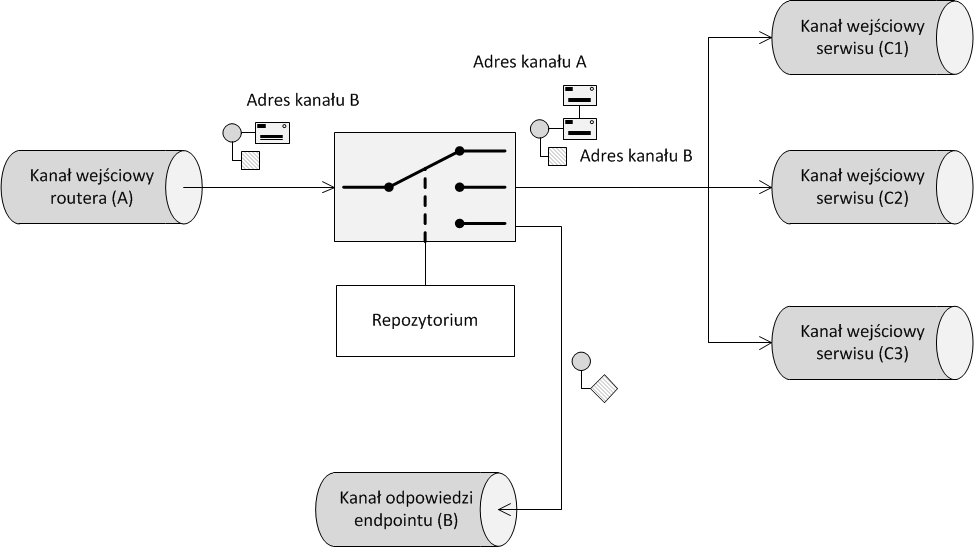
\includegraphics[scale=0.55]{router_flow.png}
	\caption{Diagram przepływu wiadomości w warstwie \textit{Routing Layer}}\label{fig:routing_layer_project}
\end{figure}

\begin{figure}[!h]
	\centering
	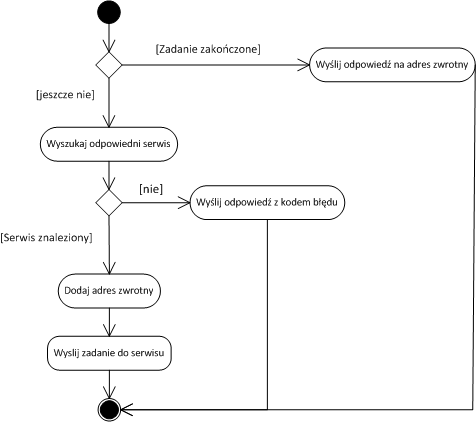
\includegraphics[scale=0.75]{router_activity.png}
	\caption{Diagram czynności komponentu routującego. }\label{fig:router_activity_diagram}
\end{figure}

\subsubsection*{Przepływ wiadomości asynchronicznych}
W celu obsługi wiadomości w sposób asynchroniczny, jeżeli wykorzystywany punkt końcowy nie zapewnia wparcia dla takiej komunikacji, należy poprzedzić proces routowania dodatkowymi krokami.
Diagram \ref{fig:asynchronous_detour} przedstawia rozwiązanie zastosowane w SpeechProcessingPlatform. Ważnym aspektem w prezentowanej koncepcji jest wprowadzenie dodatkowego typu komponentów, przechowywania danych, których zadaniem jest przechowywanie odpowiedzi pod odpowiednim kluczem. Pierwszym etapem jest rozdzielenie wiadomości na dwie grupy synchroniczne i asynchroniczne. Podział ten jest dokonywany na podstawie oznaczenia wykonanego przez punkt końcowy zlecający, a także na podstawie obecności chociaż jednego komponentu przechowywania danych. Jeżeli chociaż jeden z tych warunków nie jest spełniony żądanie będzie obsłużony w sposób opisany w poprzednim podrozdziale. Jeżeli obydwa warunki są spełnione wiadomość jest poddawana kilku dodatkowym operacjom przed wysłaniem jej do routera. Pierwsza z nich to usunięcie oznaczenia do przetwarzania asynchronicznego. Druga to wygenerowanie i dodanie do wiadomości unikalnego identyfikatora, który posłuży jako klucz przy przechowywaniu docelowej odpowiedzi. Następnym krokiem jest wygenerowanie zastępczej odpowiedzi i wysłanie jej do punktu końcowego. Odpowiedz ta zawiera wygenerowany wcześniej identyfikator, który pozwoli aplikacji klienckiej na odpytanie systemu o odpowiedź na oryginalne zadanie. Ostatnim krokiem jest podmiana adresu zwrotnego w oryginalnej wiadomości na adres komponentu przechowywania danych, do którego to odpowiedź zostanie wysłana po zakończonym przetwarzaniu.  Dalsze przetwarzanie wygląda tak samo jak w wypadku wiadomości synchronicznych.


 % mozna dodać obrazek do correlation idetifier po słowach : ...nagłówki: unikalny idetyfikator, oraz....

\begin{figure}[!h]
	\centering
	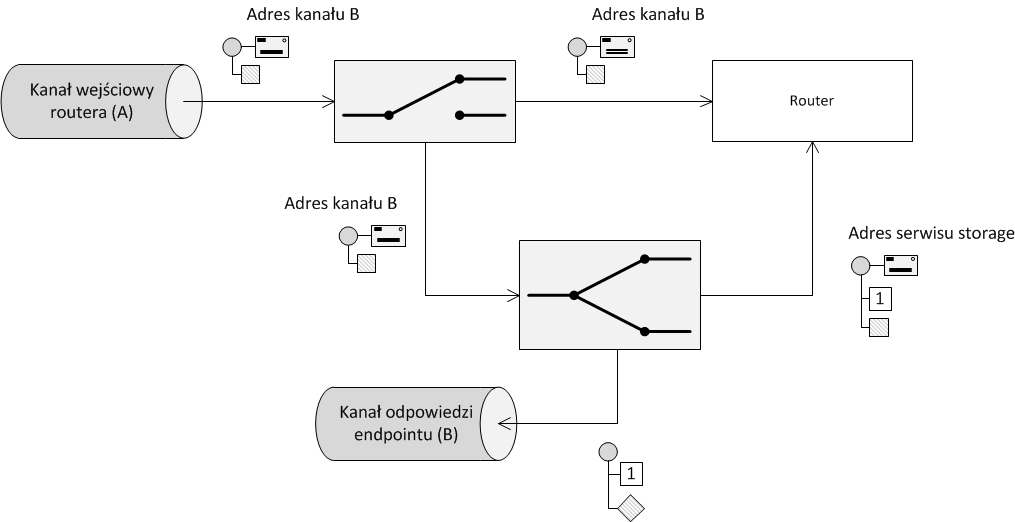
\includegraphics[scale=0.55]{asynchronous_detour.png}
	\caption{Diagram przepływu dla komunikacji asynchronicznej}\label{fig:asynchronous_detour}
\end{figure}

\begin{figure}[!h]
	\centering
	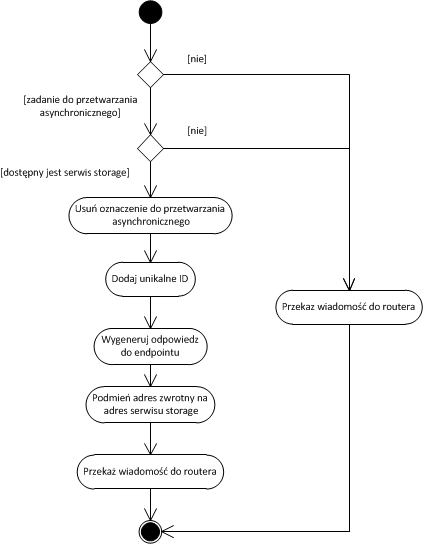
\includegraphics[scale=1.0]{asynchronous_activity_uml.png}
	\caption{Diagram czynności dla wiadomości asynchronicznych. }\label{fig:asynchronous_activity}
\end{figure}

\subsection{Warstwa \textit{Services Layer}}

Pierwszym komponentem z warstwy \textit{Services Layer}, który bierze udział podczas przetwarzania wiadomości jest repozytorium. Użycie tego komponentu nie jest wymagane , jednak jego brak wymusiłby zapisanie gdzieś w implementacji warstwy \textit{Routing Layer} stałych ścieżek lub zestawu reguł na podstawie których podejmowana byłaby decyzja o dalszej trasie wiadomości. Takie podejście mocno związałoby platformę z konkretnymi komponentami odpowiedzialnymi za przetwarzanie mowy, a dodanie nowego komponentu wiązało by się ze zmianą implementacji. Dzięki zastosowaniu repozytorium, które wprowadza dodatkową warstwę abstrakcji nad konkretnymi komponentami syntezy mowy, całość systemu nie jest związana z konkretnym dostawcą usług syntezy. Dodatkowym plusem takiego rozwiązania jest możliwość dynamicznego wyboru komponentów w zależności od zmieniających się warunków zewnętrznych. Platformę można rozszerzyć o komponenty monitorujące zachowanie się komponentów w czasie rzeczywistym co pozwoli na wybór najlepszej instancji w danym momencie. 
Aby nie wiązać platformy z konkretną implementacją repozytorium został wprowadzony interfejs, który musi być zaimplementowany przez komponenty chcące pełnić role repozytorium. Takie podejście pozwoli na użycie różnych implementacji opartych na rozmaitych technologiach jak np. Spring czy OSGi. Fragment kodu \ref{lst:repository_interface} przedstawia omawiany interfejs:

\lstset{language=Java, tabsize=4, caption=Definicja interfejsu ISreviceRepository w języku Java.,label=lst:repository_interface}

\begin{center}
\begin{lstlisting}
public interface SreviceRepository {
	Collection<String> lookupServicesURIs(Class type);
	Collection<String> lookupServicesURIs(Class type, Map<String, String> metaData);
	String lookupServiceURI(Class type);
	String lookupServiceURI(Class type, Map<String, String> metaData);
}
\end{lstlisting}
\end{center}

Chociaż repozytorium komponentów jest ważną częścią systemu to nie bierze ono czynnego udziału w przetwarzaniu wiadomości. Adres komponentu który zostaje zwrócony jako odpowiedź na żądanie routera służy do wysłania zadania do odpowiedniej instancji. Diagram \ref{fig:services_layer_project} przedstawia przepływ wiadomości w warstwie \textit{Services Layer}. Przepływ ten jest stosunkowo prosty. Wiadomości pojawiające się w kanale wejściowym są odbierane i poddawane przetwarzaniu. Odpowiedź odsyłana jest na adres zwrotny zawarty w wiadomości, który zawsze wskazuje na adres kanału wejściowego routera. 

\begin{figure}[!h]
	\centering
	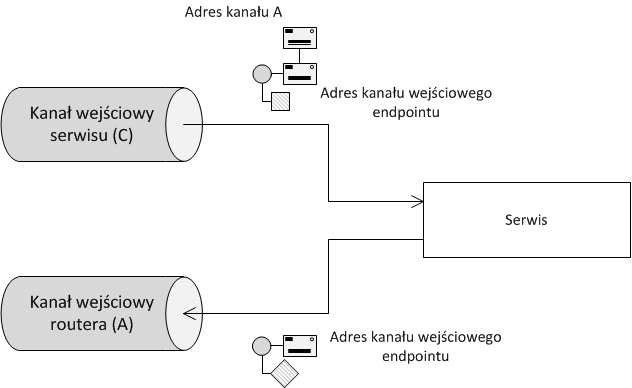
\includegraphics[scale=0.85]{services_layer_flow.png}
	\caption{Diagram przepływu wiadomości w warstwie \textit{Services Layer}}\label{fig:services_layer_project}
\end{figure}

Pierwszym wymaganiem stawianym konkretnym instancjom komponentów przetwarzających mowę jest implementacja interfejsu \textit{MessageEnabledService} \ref{lst:service_interface}. Interfejs ten posiada tylko jedną metodę, która zwraca adres kanału wejściowego danego komponentu. Spełnienie tego wymagania jest konieczne aby repozytorium było w stanie odnaleźć komponent i zwrócić jego adres routerowi, jednak aby dana instancja pełniła jakąkolwiek rolę w systemie musi także udostępniać informację o funkcjonalności przez niej dostarczanej. W tym celu instancje muszą implementować dodatkowe interfejsy, które jednoznacznie określają udostępnianą funkcjonalność. Ponieważ komunikacja między komponentami przetwarzania mowy, a resztą systemu odbywa się przez kanały wiadomości, interfejsy te służą tylko do oznaczenia komponentów a nie jako kontrakt miedzy nimi a, innymi komponentami z nich korzystającymi. Takie użycie interfejsu jest znane jako wzorzec \textit{Marker interface} \cite{bloch2008}.

\lstset{language=Java, tabsize=4, caption=Definicja interfejsu MessageEnabledService w języku Java.,label=lst:service_interface}

\begin{center}
\begin{lstlisting}
public interface MessageEnabledService {
	String getServiceURI();
}
\end{lstlisting}
\end{center}

Jak było wspomniane wcześniej, komponenty syntezy mowy zostały podzielone na 5 podstawowych grup, lecz nic nie stoi na przeszkodzie aby dodać kolejne, tak jak to ma miejsce z komponentami przechowywania danych. Jedyne co trzeba zrobić to zarejestrować komponent pod odpowiednim interfejsem. Fragment kodu \ref{lst:services_interfaces} przedstawia 5 interfejsów syntezy mowy plus interfejs przechowywania danych.

\lstset{language=Java, tabsize=4, caption=Definicja interfejsów komponentów dostarczających usługi przetwarzania mowy i przechowywania danych w języku Java.,label=lst:services_interfaces}

\begin{center}
\begin{lstlisting}

public interface OCRService {
}

public interface TTSService {
}

public interface ASRService {
}

public interface TranslationService {
}

public interface LanguageRecognitionService {
}

public interface StorageService {
}
\end{lstlisting}
\end{center}

Drugim i ostatnim wymaganiem stawianym przed implementacjami usług przetwarzania mowy jest obsługa wiadomości w wewnętrznym formacie używanym przez resztę komponentów systemu. Jest to spowodowane brakiem informacji na temat formatu wiadomości obsługiwanego przez dany komponent. Podczas procesu routowania, znany jest tylko adres i typ docelowego komponentu, dlatego router nie jest w stanie przetransformować wiadomości do obsługiwanego formatu. 


Aby możliwe było użycie gotowych usług, które nie obsługują komunikacji opartej o wiadomości należy użyć komponenty które będą działać na zasadzie proxy i to one będą rejestrować się w rejestrze komponentów. Po otrzymaniu wiadomości komponent proxy, podda ją wymaganej transformacji po czym wyśle zadanie do konkretnej instancji usługi, używając przy tym odpowiedniego adaptera, jeżeli zajdzie taka potrzeba. 

\begin{figure}[!h]
	\centering
	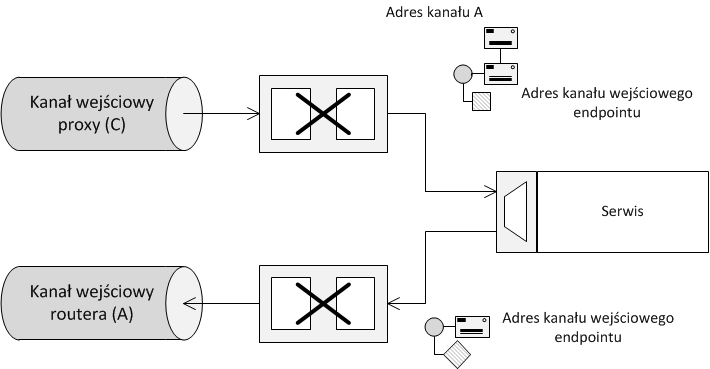
\includegraphics[scale=0.8]{proxy_layer_flow.png}
	\caption{Proxy wraz z elementami transformującymi oraz adapterem. }\label{fig:servis_proxy}
\end{figure}


\section{Implementacja}

Do implementacji systemu SpeechProcessingPlatform została użyta platforma integracyjna Apache ServiceMix, która w znaczący sposób ułatwia rozwiązywanie problemów integracji, dzięki dostarczaniu dużej ilości gotowych komponentów. Zastosowanie kontenera OSGi, na którym platforma ta jest oparta, pozawala na dynamiczną adaptację systemu w zależności od zaistniałych warunków. Dodatkowo pozwala podzielić system na niezależne, wymienialne części (bundle), z których każda posiada niezależny od reszty cykl życia. Dodawanie nowych części, takich jak kolejne punkty końcowe, czy kolejne komponenty udostępniające usługi przetwarzania mowy może być realizowane w trakcie pracy systemu i nie wymaga jego ponownego uruchomienia \cite{hall2011}. Do implementacji przepływów wiadomości został użyty Apache Camel, który jest jedną z części składowych ServiceMix-a. Framework ten zawiera bardzo dużą liczbę wbudowanych punktów końcowych, obsługujących większość z popularnych protokołów komunikacji takich jak: FTP, HTTP, IMAP czy XMPP. Dzięki temu dodanie obsługi większej ilości protokołów nie stanowi żadnego problemu. Framework ten, pozwala również w prosty w sposób zaimplementować większość wzorców EIP, dlatego implementacja opisanych w poprzednim podrozdziale przepływów wiadomości jest stosunkowo prosta.

\subsection{Wewnętrzny format wiadomości}
Wiadomości przesyłane wewnątrz systemu mają postać obiektów. Obiekty te posiadają wszystkie potrzebne informacje aby można było przeprowadzić przetwarzanie, czyli typ przetwarzanie, dane wejściowe i parametry przetwarzania. Wynik przetwarzania jest również przechowywany w obiekcie wiadomości, dzięki czemu może on posłużyć jako dane wejściowe dla kolejnego etapu albo jako wynik końcowy całego procesu. Takie podejście ułatwia operacje na wiadomościach, np. sprawdzenie czy zadanie jest już zakończone sprowadza się do wywołania metody. Fragment kodu \ref{lst:task_interface} przedstawia interfejs który musi być implementowany przez obiekty wiadomości.

\lstset{language=Java, tabsize=4, caption=Definicja interfejsu Task w języku Java.,label=lst:task_interface}

\begin{center}
\begin{lstlisting}
public interface Task {
	boolean isFinished();
	boolean isAsynchronous();
	Class getRequiredServiceType();
	Map<String, String> getMetaData();
	String getReturnAddress();
	void addReturnAddress(String address);
	Object getInputData();
	void setOuputData(Object data);
}
\end{lstlisting}
\end{center}

Zadania mogą mieć postać jedno lub wieloetapową, lecz fakt ten powinien być nie widoczny dla komponentów systemu. Jest to klasyczny przykład na zastosowanie wzorca projektowego kompozyt(diagram \ref{fig:composite_pattern}), który jest szeroko stosowany w informatyce, a szczegółowo opisany chociażby w \cite{gamma1995}.

\begin{figure}[!h]
	\centering
	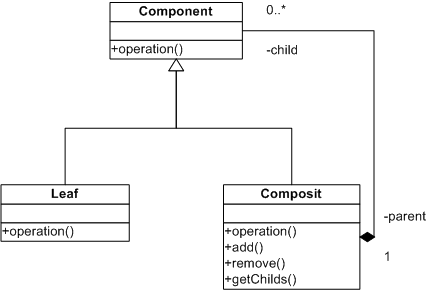
\includegraphics[scale=0.7]{composit_pattern.png}
	\caption{Wzorzec kompozyt}\label{fig:composite_pattern}
\end{figure}

Każdy z opisanych wcześniej rodzajów przetwarzania mowy posiada swoją klasę obiektów reprezentująca zadania danego typu. Diagram \ref {fig:task_class_hierarchy} przedstawia strukturę dziedziczenia klas reprezentujących obiekty zadań. Przedstawiona została tylko klasa zadań TTS, pozostałe klasy są analogiczne. 

\begin{figure}[!h]
	\centering
	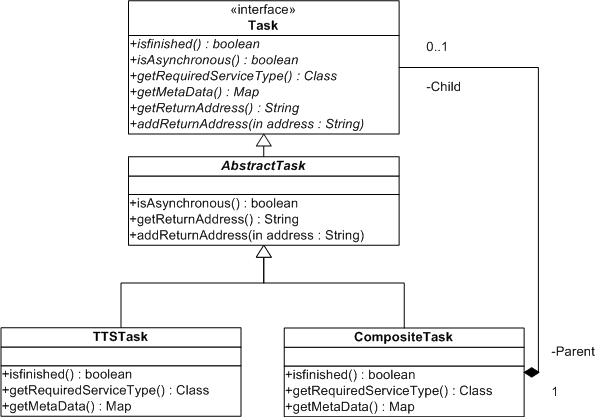
\includegraphics[scale=0.65]{tasks_hierarhy.png}
	\caption{Struktura dziedziiczenia klasy Task}\label{fig:task_class_hierarchy}
\end{figure}


\subsection{Warstwa \textit{Data Endpoints Layer}}

Dzięki bogatej bazie komponentów dostępnych w Apache Camel, implementacja konkretnych punktów końcowych sprowadza się raczej do konfiguracji. W większości przypadków jedyne co trzeba zrobić to dostarczyć odpowiedni adres URI, który pozwoli frameworkowi stworzyć i uruchomić wymagany punkt końcowy. Fragment kodu \ref{lst:camel_uris} przedstawia przykładowe formaty adresów URI

\lstset{language=Java, tabsize=4, caption=Przykładowe formaty adresów URI dla punktów końcowych Apache Camel.,label=lst:camel_uris}
\begin{minipage}{\linewidth}
\begin{center}
\begin{lstlisting}
	ftp://[username@]hostname[:port]/directoryname[?options]
	smtp://[username@]host[:port][?options]
	jms:[queue:|topic:]destinationName[?options]
	cxf:bean:cxfEndpoint[?options]
	cxfrs:bean:rsEndpoint[?options]
\end{lstlisting}
\end{center}
\end{minipage}

Aby użyć niektórych rodzajów punktów końcowych, wymagany nakład pracy jest trochę większy, lecz nadal stosunkowo mały. Chcąc udostępnić system za pomocą technologii Web services należało stworzyć również opis usługi, jednak sprowadza się to do implementacji prostego interfejsu z dodatkowymi adnotacjami.  Fragment kodu \ref{lst:rest_service} przedstawia definicje usługi zgodnej z technologią REST web services, która zastała użyta do konfiguracji punktu końcowego cxfrs. Metody w poniższej klasie nie są wywoływane, służą one tylko do konfiguracji punktu końcowego. Za całe przetwarzanie odpowiedzialna jest reszta ścieżki Apache Camel.


\lstset{language=Java, tabsize=4, caption=Definicja REST-owego punktu końcowego.,label=lst:rest_service}


%Trzeba to przejrzeć czy to działa zanim to sie pokaże wiekszej liczbie osób.
\begin{center}
\begin{lstlisting}
@Path("/speech_processing/rest")
public class RESTSpeechProcessingService {

	@POST
	@Path("/process")
    	public Response process(@FormParam("task")  String task, @FormParam("input")  File input) {
		return null;
	}

	@GET
	@PATH("/get_response")
	public Response getResponse(@QueryParam("id")  String responseId) {
		return null;
	}
}

\end{lstlisting}
\end{center}

Po odebraniu wiadomości przez punkt końcowy kolejnym krokiem jest jej transformacja do używanego wewnętrznie formatu. Wspieranie transformacji między różnymi formatami danych jest jednym z podstawowych wymagań stawianych przed rozwiązaniami ESB, dlatego też w ServiceMix-ie problem ten posiada bardzo duże wsparcie ze strony frameworku. Apache Camel udostępnia zbiór gotowych komponentów, dzięki którym transformacja między formatami takimi jak JSON, XML, czy CSV staje się trywialna. Jeżeli jednak, transformacja nie jest standardowa, framework posiada konstrukcje, które w łatwy sposób umożliwiają dodanie własnych komponentów transformujących. W przypadku transformacji wiadomości otrzymanych przez punkty końcowe, transformacja polega na zamianie opisu zadania w postaci pliku XML, na obiekt przedstawiający odpowiednie zadanie. Do tego zadania wykorzystano technologie JAXB \cite{jaxb2008}. Pozwala ona w prosty i przejrzysty sposób opisać mapowanie obiekt \begin{math}\Leftrightarrow\end{math} xml przy pomocy zestawu adnotacji. Dzięki zachowaniu odpowiedniej konwencji nazewnictwa opisanie mapowania sprowadza się do dodania tylko jednej adnotacji do każdej z klas opisujących zadania. Fragment kodu \ref{lst:jaxb_annotation} przedstawia klasę TTSTask z dodaną adnotacją JAXB.


% TO TEZ SPRAWDZIC , CZY ZADZIALA ZE ZLOZONYMI TYPAMI
\lstset{language=Java, tabsize=4, caption=Definicja klasy TTSTask wraz z adnotacjami JAXB .,label=lst:jaxb_annotation}

\begin{center}
\begin{lstlisting}
@XmlRootElement(name="tts")
public class TTSTask extends AbstarctTask {
	...
}
\end{lstlisting}
\end{center}

Ostatnim zadaniem punktu końcowego jest przesłanie gotowej wiadomości do routera. Jedyne czego do tego potrzebuje to adres URI kanału wejściowego routera. Adres ten jest dostarczany za pomocą pliku konfiguracyjnego. Takie rozwiązanie nie pozwala na dynamiczną zmianę ścieżki, lecz nie jest to wymagane ponieważ bez routera, reszta komponentów nie może pełnić swojej roli.
Fragment kodu \ref{lst:email_endpoint} przedstawia kompletną implementację przepływu wiadomości od punktu końcowego do routera.

\lstset{language=XML, tabsize=4, caption=Przykładowa\, kompletna implementacja przypływu wiadomości od punktu końcowego do routera przy pomocy XML DSL.,label=lst:email_endpoint}

\begin{center}
\begin{lstlisting}

<camelContext xmlns="http://camel.apache.org/schema/spring">

	<dataFormats>
		<jaxb id="jaxb" contextPath="pl.edu.agh.speechprocessing.tasks"/>
	</dataFormats>

	<route>
		<from uri="smtp://gmail.com?password=pass123&username=SpeechProcessingPlatform"/>
		<unmarshal ref="jaxb"/>
		<to uri="{{routerURI}}" />
	</route>

</camelContext>
\end{lstlisting}
\end{center}


\subsection{Warstwa \textit{Routing Layer}}

Najważniejszym elementem tej warstwy jak i całego systemu jest router. Jedyną zależnością pomiędzy routerem a innymi komponentami systemu jest jego adres, dzięki czemu system jest bardzo słabo powiązany z konkretną implementacją komponentu routującego, dzięki czemu implementacje te można dowolnie podmieniać stosownie do zaistniałych potrzeb. Apache Camel bardzo upraszcza proces implementacji routera. Dzięki użyciu elementu \textit{dynamicRouter} jedyne co zostaje do implementacji to metoda zwracająca odpowiedni adres URI. Ponieważ \textit{dynamicRouter} musi być ostatnim elementem ścieżki, ustawienie poprawnego adresu zwrotnego musi zostać podzielone na dwa etapy. Pierwszy etap następuje przed etapem routowania i polega na dodaniu adresu zwrotnego routera niezależnie od tego gdzie ostatecznie wiadomość zostanie przesłana. Drugi etap polega na usunięciu adresu routera z wiadomości i następuje tylko jeżeli proces przetwarzania został zakończony, czyli jeżeli wszystkie wymagane kroki zostały wykonane albo któryś z nich nie może zostać wykonany z powodu braku odpowiedniego komponentu. Poniżej przedstawiona została przykładowa ścieżka Apache Camel odpowiadająca za przepływ wiadomości w opisywanej warstwie jak i przykładowa implementacja komponentu routującego.

\lstset{language=XML, tabsize=4, caption=Scieżka Apache Camel odpowiadająca za przepływ wiadomości w warstwie \textit{Routing Layer}.,label=lst:routin_layer_impl}

%SPRAWDZIĆ
\begin{center}
\begin{lstlisting}

<bean id="dynamicRouter" class="pl.edu.agh.speechprocessing.routing.DynamicRouter"/>

<camelContext xmlns="http://camel.apache.org/schema/spring">

	<route>
		<from uri="{{routerURI}}" />
		<bean ref="dynamicRouter" method="addRouterAddress"/>
		<dynamicRouter>
			<method ref="dynamicRouter" method="route" />
		</dynamicRouter>
	</route>


	<route>
		<from uri="direct:responseChannel">
		<bean ref="dynamicRouter" method="removeRouterAddress"/>
		<dynamicRouter>
			<method ref="dynamicRouter" method="routeResponse" />
		</dynamicRouter>
	</route>

</camelContext>

\end{lstlisting}
\end{center}

\lstset{language=Java, tabsize=4, caption=Implementacja metody routującej wiadomości do odpowiednich komponentów przetwarzania mowy.,label=lst:router_impl}

\begin{center}
\begin{lstlisting}

class DynamicRouter {

	...

	public String route(Task task) {
		if (task.isFinished()) {
			return "direct:responseChannel";
		} else {
			//jezeli zostal znaleziony serwis to zwracamy jego adres
			String uri = serviceRepository.lookupServiceURI(task.getRequiredServiceType(), task.getMetaData());
			if (service != null) {
				return uri;
			} else {
				return "direct:responseChannel";
			}
		}
	}

	public String routeResponse(Task task) {
		return task.getReturnAddress();
	}


	public Task removeRouterAddress(Task task) {
		//usuniecie adresu routera z listy adresow zwrotnych
		task.getReturnAddress();
		return task;
	}


	public Task addRouterAddress(Task task) {
		//dodanie adresu routera do listy adresow zwrotnych
		task.addReturnAddress(getRouterAddress());
		return task;
	}

	...
}
\end{lstlisting}
\end{center}

\subsection{Warstwa \textit{Services Layer}}

Implementacja repozytorium zastosowana w systemie SpeechProcessingPlatform jest oparta na technologii OSGi, lecz dzięki dobrze wyspecifikowanemu interfejsowi, system ten nie jest związany z tą jedną, konkretną implementacją. Bazowanie na kontenerze OSGi pozwala dodać dynamiczną naturę do systemu. Takie podejście pozwala dodawać nowe komponenty bez zatrzymywania systemu. Ponieważ OSGi posiada wbudowany rejestr usług, więc cała logika związana z rejestrowaniem się i utrzymywaniem listy dostępnych komponentów jest zapewniona, jedyne co zostaje do zaimplementowania to proces odpytywania rejestru o odpowiedni komponent. Podstawowym typem wyszukiwania jakie udostępnia rejestr OSGi jest wyszukiwanie po typie usługi. Dodatkowo udostępnia on metodę wyszukiwania, która przyjmuje standardowy filtr LDAP \cite{ldaprfc1996} w postaci ciągu znaków. Rejestr OSGi porównuje parametry z filtru z parametrami w definicji usługi i na tej podstawie podejmuje decyzję które adresy do komponentów zwrócić. Fragment \ref{lst:ldap_tts_query} przedstawia przykładowe zapytania LDAP zawierające parametry dotyczące przetwarzania mowy. Oprócz opisu usług w postaci typu oraz parametrów, OSGi pozwala również na nadawanie im rankingu, dzięki czemu jeżeli więcej niż jedna usługa spełnia zadane wymagania, pozwala zdecydować która usługa jest lepszy. Kompletny algorytm wyboru najlepiej pasującej usługi można znaleźć w \cite{hall2011}. Fragment kodu \ref{lst:service_repository_impl} przedstawia klasę OSGIServiceRepository, która pełni funkcję fasady nad rejestrem wbudowanym w OSGi.

\lstset{language=Java, tabsize=4, caption=Przykładowe zapytania LDAP zawierające parametry dotyczące usług przetwarzania mowy. ,label=lst:ldap_tts_query}

\begin{center}
\begin{lstlisting}

//zapytanie o usluge TTS
"(&(language=en)(codec=mp3))"

/zaptanie o usluge OCR
"(&(language=pl)(|(imageFormat=jpg)(imageFormat=jpeg)))"


\end{lstlisting}
\end{center}

\lstset{language=Java, tabsize=4, caption=Częściowa definicja klasy OSGIServiceRepository będącą fasadą nad Rejestrem OSGi. ,label=lst:service_repository_impl}

\begin{center}
\begin{lstlisting}
public class TTSTask implements SreviceRepository{
	private BundleContext bundleContext;
	...
	
	public Collection<String> lookupServicesURIs(Class type) {
		ServiceReference[] refList = bundleContext.getServiceReferences(type.getName())
		return prepareURIsList(refList);
	}

	public Collection<String> lookupServicesURIs(Class type, Map<String, String> metaData) {
		ServiceReference[] refList = bundleContext.getServiceReferences(type.getName(), preapreFilterQuery(metaData));
		return prepareURIsList(refList);
	}

	...
}

\end{lstlisting}
\end{center}
% MOZNA DODAC REFERENCJE DO LBUEPRINTA
Ostatnimi elementami systemu są konkretne komponenty dostarczające usługi przetwarzania mowy, jednak aby jakiś komponent mógł zostać użyty w systemie musi spełniać parę warunków. Pierwszym warunkiem jest umiejętność obsługi wiadomości co jest równoznaczne z udostępnianiem jakiegoś kanału wejściowego, który pozwoli na komunikację routera z daną implementacją. Drugim warunkiem jest rejestracja w rejestrze OSGi pod odpowiednimi interfejsami oraz z odpowiednimi parametrami, co pozwoli na wyszukanie komponentu podczas procesu routowania. W celu rejestracji komponentów jako usług OSGi został użyty kontener Blueprint, który jest dostarczony razem z frameworkiem OSGi. Pozwala on na łatwą i przejrzystą definicję usług za pomocą plików konfiguracyjnych w formacie xml. Oprócz tego, pozwala on również na definicję oraz wstrzykiwanie zależności co upraszcza konfiguracje systemu. Fragment kodu \ref{lst:blueprint_definition} przedstawia definicje usługi OCR przy użyciu kontenera Blueprint.

\lstset{language=XML, tabsize=4, caption=Definicja usługi OCR przy użyciu kontenera Blueprint.,label=lst:blueprint_definition}

%SPRAWDZIĆ
\begin{center}
\begin{lstlisting}
<blueprint xmlns="http://www.osgi.org/xmlns/blueprint/v1.0.0">

	 <!-- definicja beanu ktory zostanie zarejestrowany jako usluga, jako argument przyjmuje nazwe kanalu wejsciowego -->
	<bean id="freeOCRServiceImpl" class="pl.edu.agh.speechprocessing.services.FreeOCRService">
		 <argument value="direct:freeOCRService"/> 
	</bean>

	<service ref="freeOCRService" auto-export="interfaces" ranking="5">
		<service-properties>
			<entry key="language">
				<set value-type="java.lang.String">
					<value>en</value>
					<value>it</value>
					<value>pl</value>
				</set> 
			</entry>
			<entry key="imageFormat">
				<set value-type="java.lang.String">
					<value>bmp</value>
					<value>png</value>
					<value>jpg</value>
				</set> 
			</entry>
		</service-properties>
	</service>

</blueprint>

\end{lstlisting}
\end{center}

Usługi rejestrowane w rejestrze OSGi pełnią tylko pomocniczą role. Ich zadaniem jest umożliwienie wyszukiwania oraz dostarczanie adresu pod który należy wysłać wiadomość do zainteresowanych routera. Całe przetwarzanie zaczyna się po otrzymaniu wiadomości w kanale odbiorczym udostępnianym komponentu reprezentowanego przez usługę zarejestrowaną w rejestrze OSGi. Oczywiście obiekt, który jest rejestrowany może również brać czynny udział w przetwarzaniu, ale nie musi. Jako że właściwe usługi, które dokonują przetwarzania są na zewnątrz systemu, jedyne zadanie jakie pozostaje to przygotowanie wiadomości, wywołanie usługi używając odpowiedniego protokołu, przetłumaczenie odpowiedzi na format wewnętrzny i odesłanie jej do routera. 


% Można dodać fragment implementacji.

\section*{Podsumowanie} 

Powyższy rozdział przedstawił projekt i implementację przykładowej platformy integracyjnej dla przetwarzania mowy. Zastosowanie architektury z luźno powiązanymi warstwami zostawia dużo opcji do przyszłego rozwoju systemu. Prezentowany system jest też przykładem na to jak użycie wyspecjalizowanych technologii upraszcza proces integracji. Apache ServiceMix integrujący w sobie takie technologie jak OSGi czy Apache Camel pozwala budować systemu integracyjne z gotowych elementów pozwalając ich twórcom skupić się na logice przypływu danych. Zaimplementowany system należy poddać weryfikacji względem wymagań postawionych w rozdziale 2, a także sprawdzić jego wydajność w porównaniu z tradycyjnym podejściem do systemów przetwarzania mowy.


% można wrzucic obrazek całego systemu

%Jednym z rozwiązań jest użycie wzorca \textit{Correlation Identifier}\cite{eaipatterns}:

%\begin{figure}[!h]
%	\centering
%	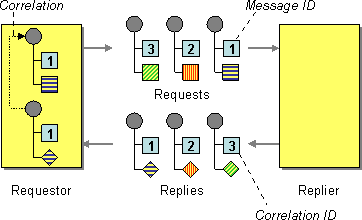
\includegraphics{CorrelationIdentifierSolution.png}
%	\caption{Wzorzec \textit{Correlation Identifier}: \url{http://www.eaipatterns.com/img/CorrelationIdentifierSolution.gif}}\label{fig:correlation_identifier}
%\end{figure}

%Endpoint po otrzymaniu żądania generuje dla niego unikalny identyfikator, który odsyła aplikacji nie czekając na wynik przetwarzania. Ten sam identyfikator jest dodawany do wiadomości %wysyłanej do routera, lecz tym razem adres zwrotny wskazuje nie na punkt końcowy lecz na serwis 



% rysunek z podziałęm na komponenty,
% rysunek EIP - ale to może być już w projekcie.
% proekt, interfejsy, chierarchie klas. 









% ---------------------------------------------------------------------------
%: ----------------------- end of thesis sub-document ------------------------
% ---------------------------------------------------------------------------

